\documentclass[c]{beamer}

\usepackage[utf8]{inputenc}
\usepackage{lmodern} 
%\usepackage[scaled=0.8]{beramono}
\usepackage[T1]{fontenc}
\usepackage{microtype}

\usepackage{graphicx}
\usepackage{float}
\usepackage[hypcap]{caption}
\usepackage{subcaption}
\usepackage{algorithm2e}
\usepackage{array}

\usepackage{media9}

\usepackage{mathtools}
\usepackage{amssymb}
\usepackage{amsthm}
\usepackage{amsmath}


\usepackage[utf8]{inputenc}
\usepackage{lmodern} 
%\usepackage[scaled=0.8]{beramono}
\usepackage[T1]{fontenc}
\usepackage{microtype}

\usepackage{graphicx}
\usepackage{float}
\usepackage[hypcap]{caption}
\usepackage{subcaption}
\usepackage{algorithm2e}
\usepackage{array}

\usepackage{media9}

\usepackage{amssymb}
\usepackage{amsthm}
\usepackage{amsmath}


\usepackage{mathtools}

%\usepackage[customcolors]{hf-tikz}
%\usepackage{pgfplots}



%\usepackage{animate}
%\usepackage{movie15}

%\usepackage{epstopdf}

%\epstopdfDeclareGraphicsRule{.gif}{png}{.png}{convert gif:#1 png:\OutputFile}
%\AppendGraphicsExtensions{.gif}



\usepackage[english]{babel}
\selectlanguage{english}

\usetheme{Warsaw}
%\usetheme{CambridgeUS}
\usecolortheme{crane}
\beamertemplatenavigationsymbolsempty

\newcommand{\inred}[1]{\textcolor{red}{#1}}
\newcommand{\inblue}[1]{\textcolor{blue}{#1}}

\beamertemplatenavigationsymbolsempty
\setbeamertemplate{footline}[page number]{}

\captionsetup[figure]{labelformat=empty}


\newcommand{\Prod}[2]{(#1, #2)_{L^2}}
\newcommand{\Mat}[1]{\mathbf{#1}}

\newcommand{\dx}{\, \mathrm{d}x}
\newcommand{\deriv}[2]{\frac{\partial {#1}}{\partial {#2}}}
\newcommand{\Int}[1]{\int_0^1 {#1}\dx}
\newcommand{\Lims}[1]{\left. #1 \right|_0^1}
\newcommand{\IntE}[2]{\int_{#1}{#2}\dx}
\newcommand{\der}[1]{{#1}^\prime}
\newcommand{\Vect}[1]{\mathbf{#1}}

\newcommand{\A}[1]{\Mat{A}\big(#1\big)}
\newcommand{\Bsp}{\mathcal{B}}
\newcommand{\E}[1]{\left[\xi_{#1}, \xi_{#1 + 1}\right]}
\newcommand{\Different}[1]{\textcolor{blue}{#1}}



\title{%
Scaling Out Alternating Direction Isogeometric L2 Projections Solver}

\author{%
    \inblue{\bf Grzegorz Gurgul (AGH)} \\
    \inblue{Marcin \L{}o\'{s} (AGH)} \\
    \inblue{Danuta~Szeliga (AGH)} \\
      \inblue{\bf Maciej Paszy\'{n}ski (AGH)} }
\date{{\bf 14th U.S. National Congress on Computational Mechanics} \break \break July 17-20, 2017, Montreal, Canada}

\begin{document}

%%%%%%%%%%%%%%%%%%%%%%%%%%%

\begin{frame}
  \titlepage
\end{frame}

%%%%%%%%%%%%%%%%%%%%%%%%%%%
\begin{frame}{Agenda}

\begin{itemize}
  \item Backgroud
  \item Isogeometric L2 projections algorithm
  \item Algorithm
  \item Conclusions
\end{itemize}

\end{frame}

%%%%%%%%%%%%%%%%%%%%%%%%%%%

\begin{frame}{Background}

{\small
\begin{itemize}
  \item Isogeometric L2 projections algorithm
\end{itemize}
  \inblue{Proposed by prof. Victor Calo:} 
L. Gao, V.M. Calo, \emph{Fast Isogeometric Solvers for Explicit Dynamics}, {\bf Computer Methods in Applied Mechanics and Engineering} (2014). 
\begin{itemize}
  \item Applications to time-dependent problems
\end{itemize}
\inblue{Tumor growth simulations (C++ sequential ): }M. \L{}o\'{s}, M. Paszy\'{n}ski, A. K\l{}usek, W. Dzwinel, Application of fast isogeometric L2 projection solver for tumor simulations, {\bf Computer Methods in Applied Mechanics and Engineering} (2017) 

\inblue{Non-linear flow (Fortran+MPI, parallel ): }
M. Wo\'{z}niak, M. \L{}o\'{s}, M. Paszy\'{n}ski, L. Dalcin, V. Calo, 
Parallel fast isogeometric solvers for explicit dynamics, {\bf Computing and Informatics} (2017) 
}

\end{frame}


%%%%%%%%%%%%%%%%%%%%%%%%%%%%%%%%%%%%%%%

%%%%%%%%%%%%%%%%%%%%%%%%%%%

\begin{frame}{Background}

\begin{itemize}
  \item Improving performance of time-dependent applications of ADS
\end{itemize}

\inblue{Step 1: CUDA implementation: }\break
G. Gurgul, M. Paszy\'{n}ski, D. Szeliga, 
Open source JAVA implementation of the parallel multi-thread alternating direction isogeometric L2 projections solver for material science simulations, {\bf KomPlasTech} (2017) 

\inblue{Step 2: Object-Oriented shared memory implementation: }\break
G. Gurgul, M. Paszy\'{n}ski, D. Szeliga, 
Open source JAVA implementation of the parallel multi-thread alternating direction isogeometric L2 projections solver for material science simulations, {\bf KomPlasTech} (2017) 

\inred{Step 3: Cloud implementation: }\break
G. Gurgul, M. Paszy\'{n}ski, D. Szeliga, Scaling Out Alternating Direction Isogeometric L2 Projections Solver, 14th U.S. National Congress on Computational Mechanics


\end{frame}




%%%%%%%%%%%%%%%%%%%%%%%%%%%%%%%%%%%%%%%

%%%%%%%%%%%%%%%%%%%%%%%%%%%%%%%%%%%%%%%

\begin{frame}{Isogeometric L2 projections}


\textbf{In general:} non-stationary problem of the form

\begin{equation*}
  \partial_t u - \mathcal{L}(u) = f(x, t)
\end{equation*}

with some initial state~$u_0$ and boundary conditions
\vspace{2mm}

$\mathcal{L}$ -- well-posed linear spatial partial differential operator

Weak form:
  $\Prod{\partial_t u + \mathcal{L}u}{v} = \Prod{f}{v}$

\vspace{3mm}

Discretization:
\begin{itemize}
  \item spatial discretization: isogeometric finite element method
  \begin{equation*}
  \Prod{\partial_t u_h + \mathcal{L}u_h}{v_h} = \Prod{f}{v_h}
  \end{equation*}
  \\\vspace{2mm}
  $u_h = \sum_i \phi_i$, $v_h\in V_h=span\{\phi_1,\ldots,\phi_n\}$ (B-splines)
  \\\vspace{2mm}
  \item time discretization with explicit method 
  e.g. forward Euler scheme
  \begin{equation*}
   \mathcal{M} u_h^{(t + 1)} =
   \mathcal{M} u_h^{(t)} +
   \Delta t \left(\mathcal{L}u_h^{(t)} + \mathcal{F}\right)
\end{equation*}
\begin{equation*}
  \Prod{u_h^{(t+1)}}{v_h} =  \Prod{u_{h}^{(t)}- \Delta t * \mathcal{L}u_h^{(t)} +\Delta t * \mathcal{F}}{v_h} 
\end{equation*}
  \\\vspace{2mm}
  \item   implies isogeometric L2 projections in every time step 
  
\end{itemize}

\end{frame}



%%%%%%%%%%%%%%%%%%%%%%%%%%%

\begin{frame}{$L^2$ projections -- tensor product basis}

\begin{figure}
  \centering
  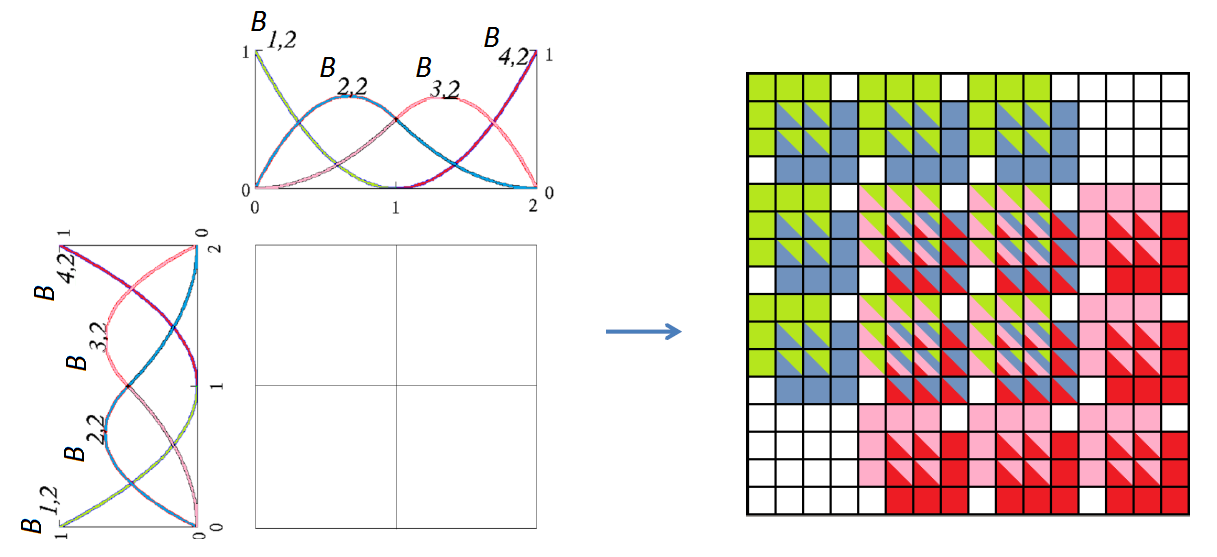
\includegraphics[width=0.8\textwidth]{img/2DFEM}
\end{figure}

Isogeometric basis functions:
\begin{itemize}
  \item 1D B-splines basis $B_1(x),\ldots, B_n(x)$
  \item higher dimensions: tensor product basis\\
        $B_{i_1\cdots i_d}(x_1,\ldots,x_d)
        \equiv B^{x_1}_{i_1}(x_1)\cdots B^{x_d}_{i_d}(x_d)$ \\
\end{itemize}
Gram matrix of B-spline basis on 2D domain $\Omega = \Omega_x \times \Omega_y$:

\begin{equation*}
  \begin{aligned}
  \mathcal{M}_{ijkl} &=
  \Prod{B_{ij}}{B_{kl}} =
  \int_\Omega B_{ij}B_{kl}\,\mbox{d}\Omega 
  \end{aligned}
\end{equation*}

Standard multi-frontal solver: $O(N^{1.5})$ in 2D, $O(N^2)$ in 3D

\end{frame}

%%%%%%%%%%%%%%%%%%%%%%%%%%%


\begin{frame}{$L^2$ projections -- tensor product basis}

Isogeometric basis functions:
\begin{itemize}
  \item 1D B-splines basis $B_1(x),\ldots, B_n(x)$
  \item higher dimensions: tensor product basis\\
        $B_{i_1\cdots i_d}(x_1,\ldots,x_d)
        \equiv B^{x_1}_{i_1}(x_1)\cdots B^{x_d}_{i_d}(x_d)$ \\
\end{itemize}
Gram matrix of B-spline basis on 2D domain $\Omega = \Omega_x \times \Omega_y$:
\begin{equation*}
  \begin{aligned}
  \mathcal{M}_{ijkl} &=
  \Prod{B_{ij}}{B_{kl}} =
  \int_\Omega B_{ij}B_{kl}\,\mbox{d}\Omega 
  \end{aligned}
\end{equation*}
 \inblue{\begin{equation*}
  \begin{aligned}
=\int_\Omega B^x_i(x) B^y_j(y) B^x_k(x) B^y_l(y) \,\mbox{d}\Omega \\
  = \int_\Omega (B_i B_k)(x)\,(B_j B_l)(y)\,\mbox{d}\Omega  \\
  = \left(\int_{\Omega_x} B_i B_k \,\mbox{d}x\right)
  \left(\int_{\Omega_y} B_j B_l \,\mbox{d}y\right) \\
  = \mathcal{M}^x_{ik} \mathcal{M}^y_{jl}
  \end{aligned}
\end{equation*}}
\begin{equation*}
\mathcal{M} = \mathcal{M}^x \otimes \mathcal{M}^y \quad\text{(Kronecker product)}
\end{equation*}

\end{frame}


%%%%%%%%%%%%%%%%%%%%%%%%%%%

\begin{frame}[fragile]{Alternating Direction Solver -- 2D}

\begin{figure}
  \centering
  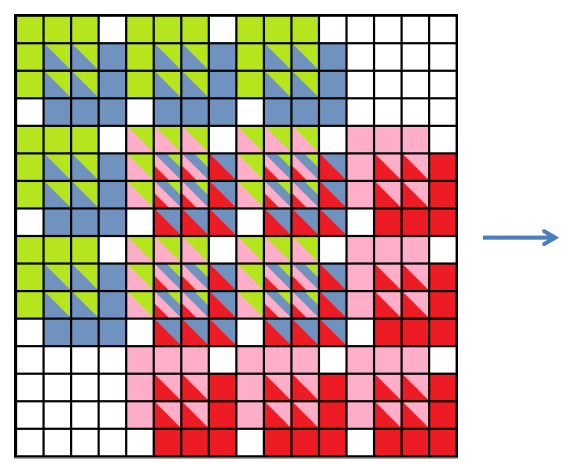
\includegraphics[width=0.4\textwidth]{img/2Dmatrix}
\end{figure}
\begin{equation*}
  \begin{bmatrix}
    A_{11} & A_{12} & \cdots & 0 \\
    A_{21} & A_{22} & \cdots & 0 \\
    \vdots & \vdots & \ddots & \vdots \\
    0 & 0 & \cdots & A_{nn} \\
  \end{bmatrix}
  \begin{bmatrix}
    y_{11} & y_{21} & \cdots & y_{m1}
    \\
    y_{12} & y_{22} & \cdots & y_{m1}
    \\
    \vdots & \vdots & \ddots & \vdots \\
    y_{1n} & y_{2n} & \cdots & y_{mn}
    \\
  \end{bmatrix}
  =
  \begin{bmatrix}
    b_{11} & b_{21} & \cdots & b_{m1} \\
    b_{12} & b_{22} & \cdots & b_{m2} \\
    \vdots & \vdots & \ddots & \vdots \\
    b_{1n} & b_{2n} & \cdots & b_{mn} \\
  \end{bmatrix}
\end{equation*}
\begin{equation*}
  \begin{bmatrix}
    B_{11} & B_{12} & \cdots & 0 \\
    B_{21} & B_{22} & \cdots & 0 \\
    \vdots & \vdots & \ddots & \vdots \\
    0 & 0 & \cdots & B_{mm} \\
  \end{bmatrix}
  \begin{bmatrix}
    x_{11} & \cdots & x_{1n} \\
    x_{21} & \cdots & x_{2n} \\
    \vdots & \ddots & \vdots \\
    x_{m1} & \cdots & x_{mn} \\
  \end{bmatrix}
  =
  \begin{bmatrix}
    y_{11} &
    y_{12} & \cdots &
    y_{1n} \\
    y_{21} & y_{22} & \cdots & y_{2n} \\
    \vdots & \vdots & \ddots & \vdots \\
    y_{m1} &
    y_{m2} & \cdots &
    y_{mn} \\
  \end{bmatrix}
\end{equation*}

\end{frame}


%%%%%%%%%%%%%%%%%%%%%%%%%%%%%%%%%%%%%%%%
%%%%%%%%%%%%%%%%%%%%%%%%%%%

\begin{frame}[fragile]{Alternating Direction Solver -- 2D}
\begin{figure}
  \centering
  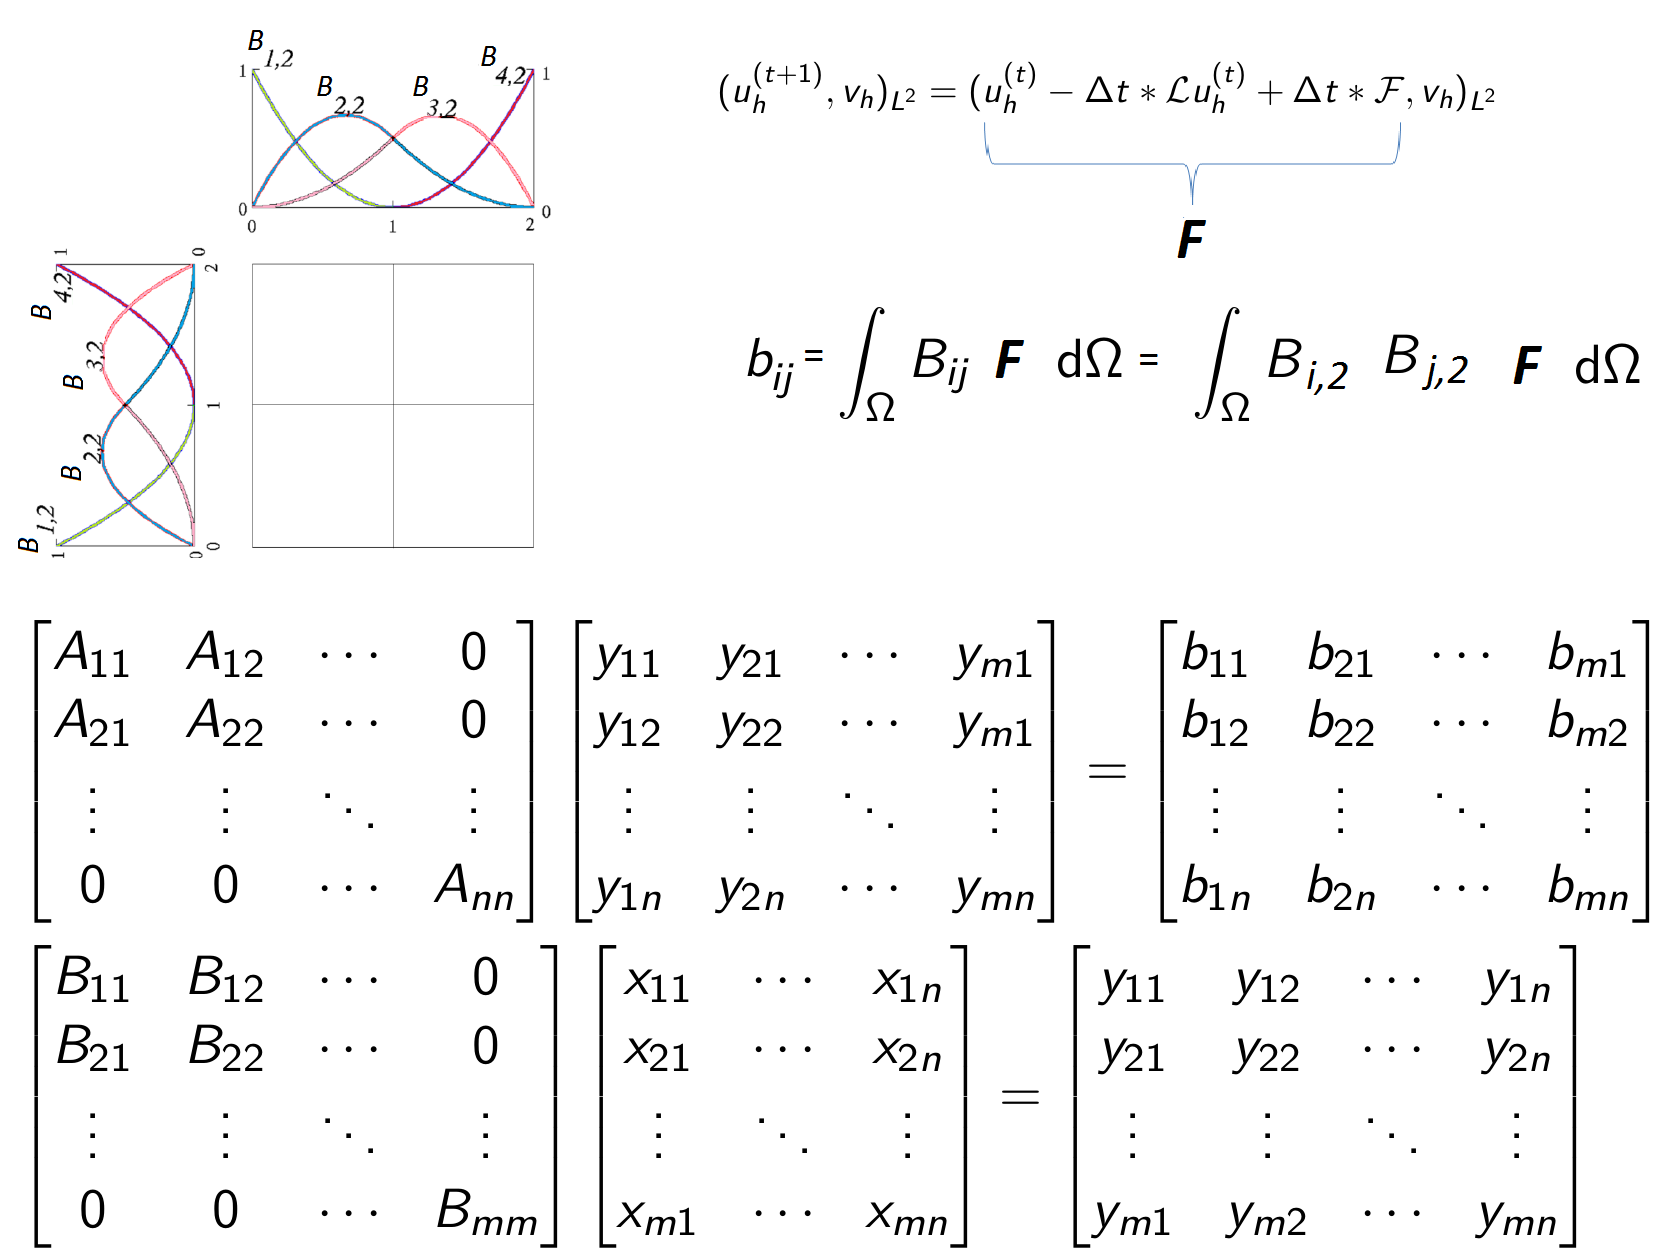
\includegraphics[width=1.0\textwidth]{img/RHS}
\end{figure}
\end{frame}
%%%%%%%%%%%%%%%%%%%%%%%%%%%

\begin{frame}{Gram matrix of tensor product basis}

\begin{figure}
  \centering
  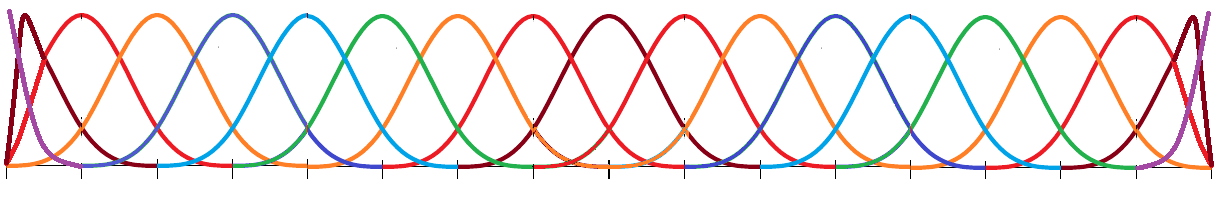
\includegraphics[width=0.6\textwidth]{img/Bsplines}
\end{figure}

B-spline basis functions have \textbf{local support} (over $p+1$ elements) 

$\mathcal{M}^x$, $\mathcal{M}^y$, \ldots -- banded structure

$\mathcal{M}^x_{ij} = 0 \iff |i - j| > 2p + 1$

Exemplary basis functions and matrix for cubics

\begin{tiny}
\begin{equation*}
	\begin{bmatrix}
    \Prod{B_1}{B_1} & \Prod{B_1}{B_2} & \Prod{B_1}{B_3} & \Prod{B_1}{B_4} & 0 & 0 & \cdots & 0 \\
    \Prod{B_2}{B_1} & \Prod{B_2}{B_2} & \Prod{B_2}{B_3} & \Prod{B_2}{B_4} & \Prod{B_2}{B_5} & 0 & \cdots & 0 \\
    \Prod{B_3}{B_1} & \Prod{B_3}{B_2} & \Prod{B_3}{B_3} & \Prod{B_3}{B_4} & \Prod{B_3}{B_5} & \Prod{B_3}{B_6} & \cdots & 0 \\
    \vdots & \vdots & \vdots & \vdots &  \vdots & \vdots &  & \vdots\\
    0 & 0 & \ldots & \Prod{B_n}{B_{n-3}}& \Prod{B_n}{B_{n-2}} & \Prod{B_n}{B_{n-1}} & \Prod{B_n}{B_n}
  \end{bmatrix}
\end{equation*}
\end{tiny}

\end{frame}




%%%%%%%%%%%%%%%%%%%%%%%%%%%

\begin{frame}[fragile]{Alternating Direction Solver -- 2D}

{Two steps} -- solving systems with $\Mat{A}$ and $\Mat{B}$ in different \emph{directions}
\begin{equation*}
  \begin{bmatrix}
    A_{11} & A_{12} & \cdots & 0 \\
    A_{21} & A_{22} & \cdots & 0 \\
    \vdots & \vdots & \ddots & \vdots \\
    0 & 0 & \cdots & A_{nn} \\
  \end{bmatrix}
  \begin{bmatrix}
    y_{11} & y_{21} & \cdots & y_{m1}
    \\
    y_{12} & y_{22} & \cdots & y_{m1}
    \\
    \vdots & \vdots & \ddots & \vdots \\
    y_{1n} & y_{2n} & \cdots & y_{mn}
    \\
  \end{bmatrix}
  =
  \begin{bmatrix}
    b_{11} & b_{21} & \cdots & b_{m1} \\
    b_{12} & b_{22} & \cdots & b_{m2} \\
    \vdots & \vdots & \ddots & \vdots \\
    b_{1n} & b_{2n} & \cdots & b_{mn} \\
  \end{bmatrix}
\end{equation*}
\begin{equation*}
  \begin{bmatrix}
    B_{11} & B_{12} & \cdots & 0 \\
    B_{21} & B_{22} & \cdots & 0 \\
    \vdots & \vdots & \ddots & \vdots \\
    0 & 0 & \cdots & B_{mm} \\
  \end{bmatrix}
  \begin{bmatrix}
    x_{11} & \cdots & x_{1n} \\
    x_{21} & \cdots & x_{2n} \\
    \vdots & \ddots & \vdots \\
    x_{m1} & \cdots & x_{mn} \\
  \end{bmatrix}
  =
  \begin{bmatrix}
    y_{11} &
    y_{12} & \cdots &
    y_{1n} \\
    y_{21} & y_{22} & \cdots & y_{2n} \\
    \vdots & \vdots & \ddots & \vdots \\
    y_{m1} &
    y_{m2} & \cdots &
    y_{mn} \\
  \end{bmatrix}
\end{equation*}

%$\Mat{A}$, $\Mat{B}$ -- multidiagonal matrices for one-dimensional bases \\
Two one dimensional problems with multiple RHS:
\begin{itemize}
\item $ n \times n $ with $m$ right hand sides $\rightarrow$ $O(n*m)=O(N)$
\item $ m \times m $ with $n$ right hand sides $\rightarrow$ $O(m*n)=O(N)$
\end{itemize}
Linear computational cost $O(N)$

\end{frame}



%%%%%%%%%%%%%%%%%%%%%%%%%%%%%%%%%%%%%%%%
%
%\begin{frame}{Isogeometric L2 projections}
%
%\inblue{The computational cost of the solver is so low,\\  that most of the time is spent on the integration} 
%
%\begin{columns}
%  \begin{column}{0.5\textwidth}
%  \begin{figure}
%      \centering
%      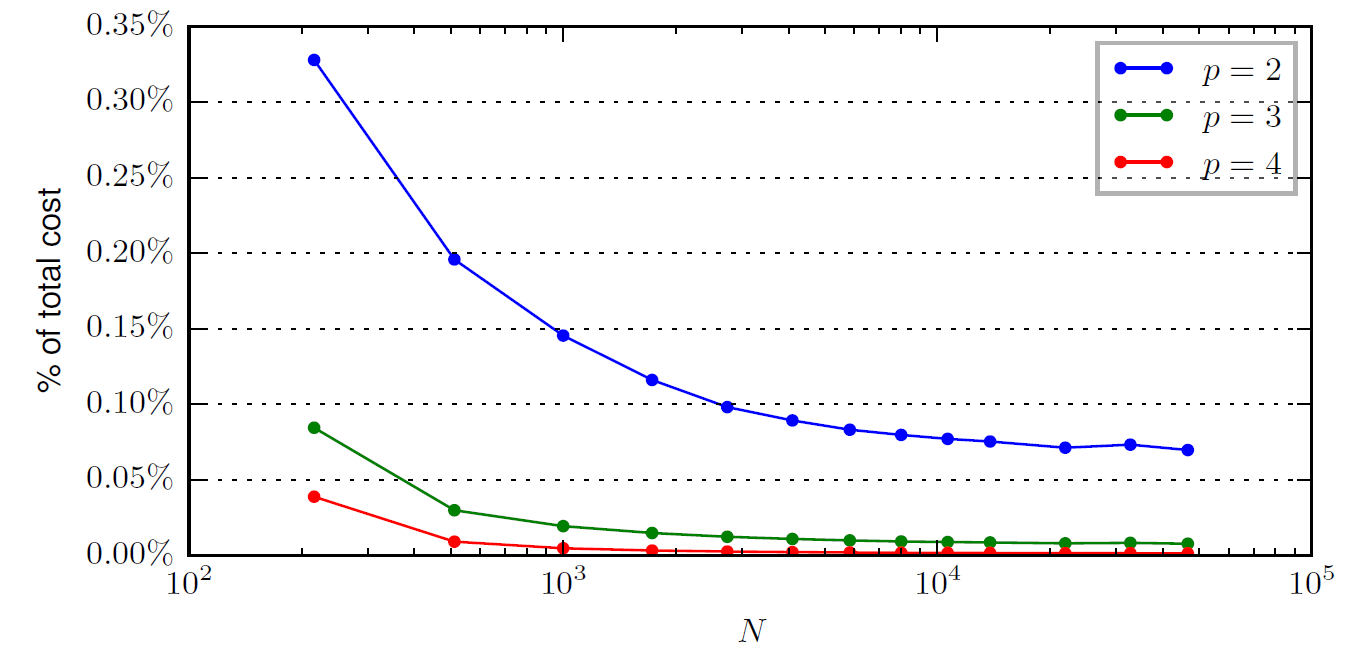
\includegraphics[width=1.1\textwidth]{img/Fraction}
%      \caption{Time spent on integration with respect to time spent on factorization (below 1 percent of the total time for 2D problems, \\ for all $p$ and $N$)}
%    \end{figure}
%  \end{column}
%
%  \begin{column}{0.5\textwidth}
%    \begin{figure}
%      \centering
%      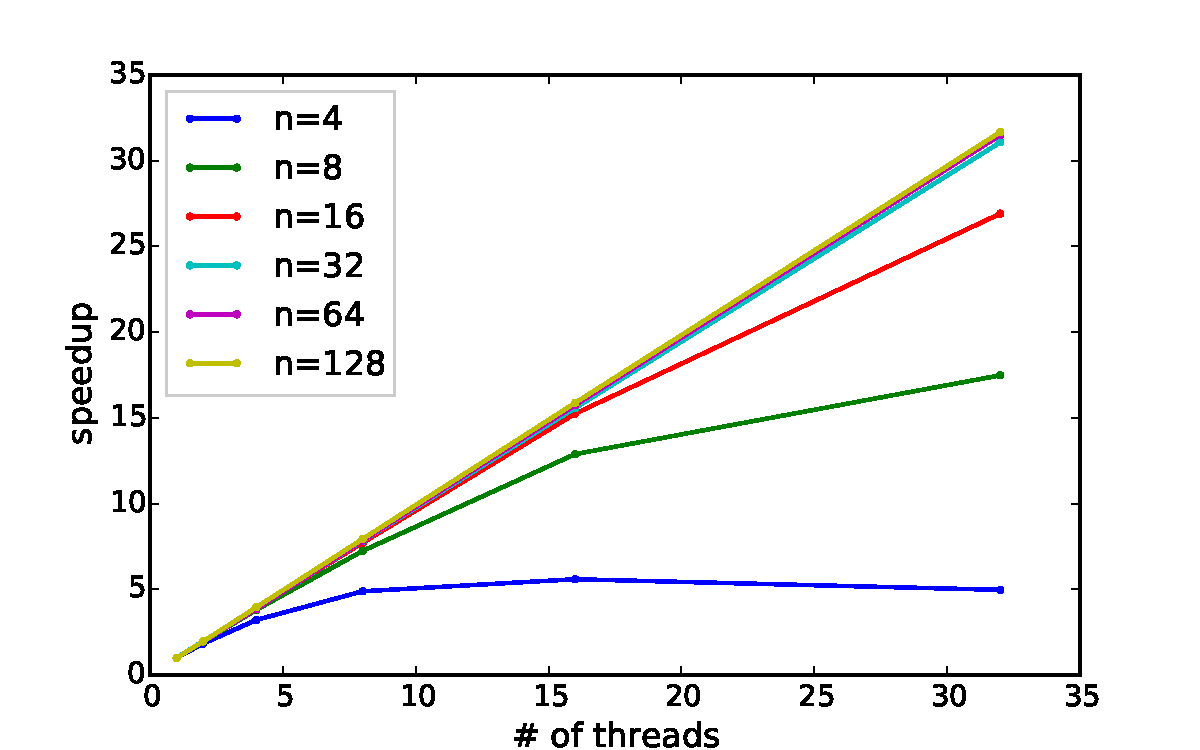
\includegraphics[width=0.95\textwidth]{img/speedup_p3}
%      \caption{Speedup of parallel integration with GALOIS \\cubics, 2D problem \\ different mesh sizes}
%    \end{figure}
%  \end{column}
%\end{columns}
%
%\inblue{Expensive isogeometric integration that can be speeded-up \\ on multi-core machines } \\
%\end{frame}
%%%%%%%%%%%%%%%%%%%%%%%%%%%


\begin{frame}{Hitting elastic material (1/2)}

    \begin{figure}
      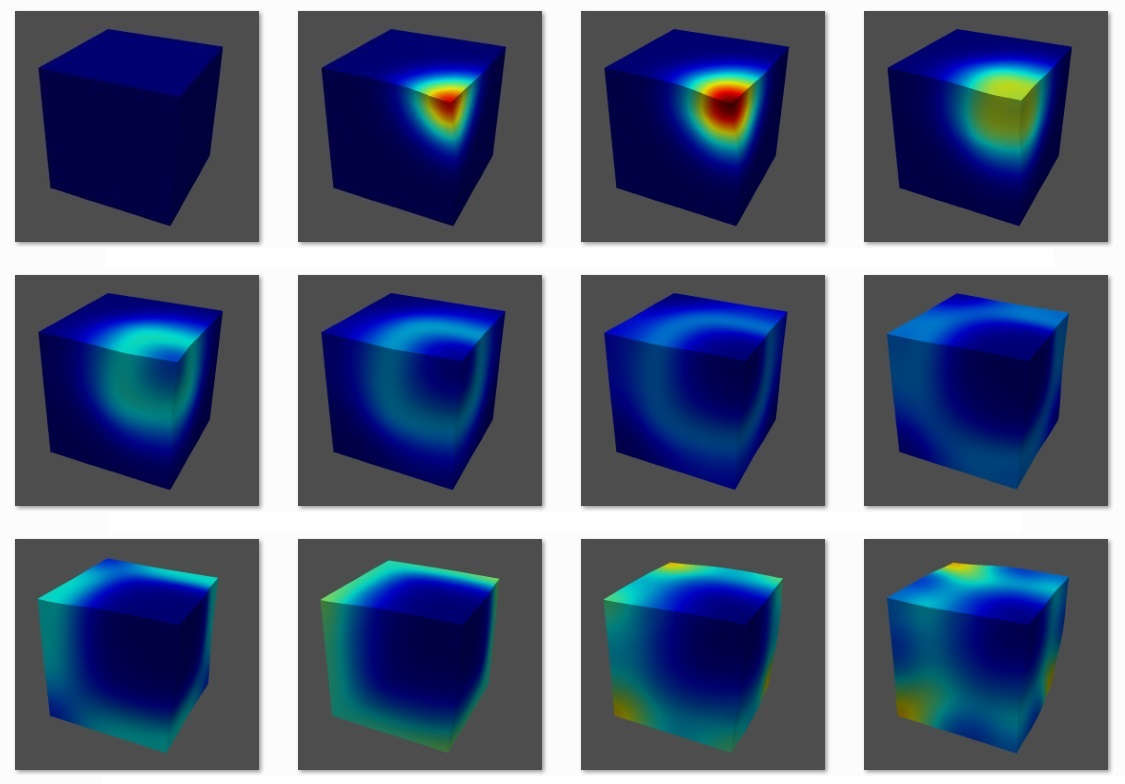
\includegraphics[width=0.95\textwidth]{img/Figure4}
      \caption{Snapshoots from the simulation }
    \end{figure}


\end{frame}

\begin{frame}{Hitting elastic material (2/2)}

    \begin{figure}
      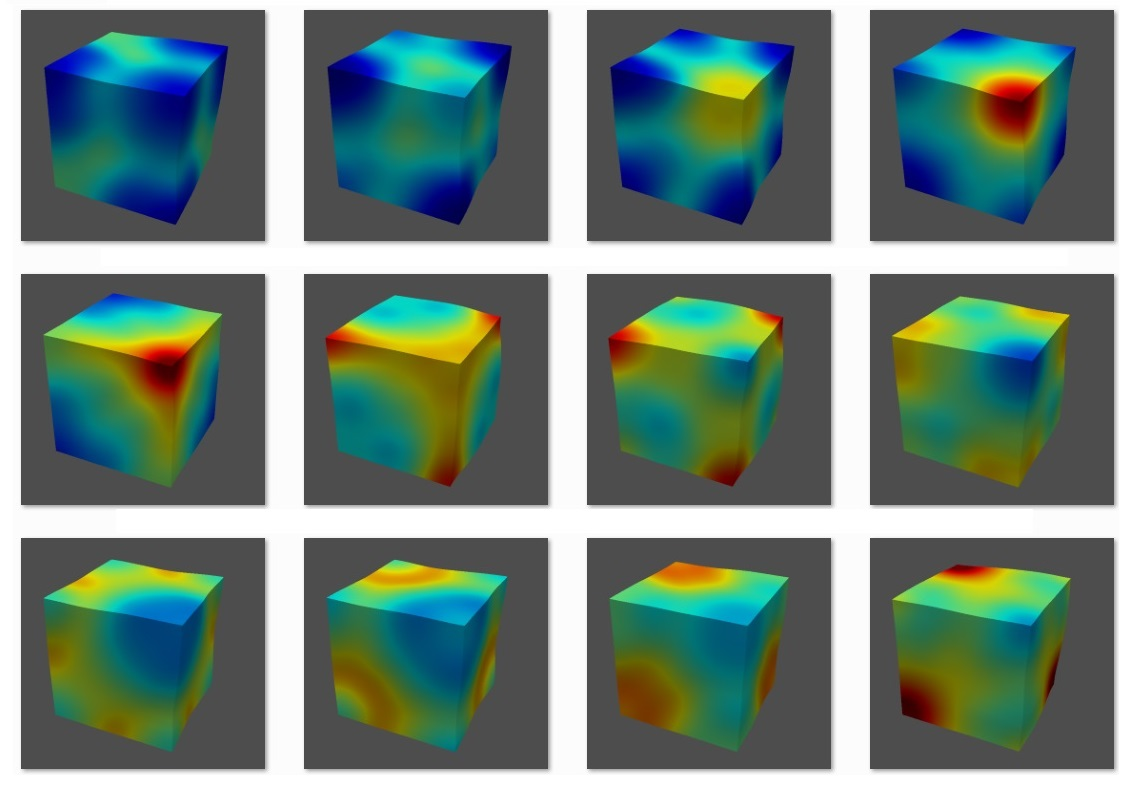
\includegraphics[width=0.95\textwidth]{img/Figure5}
      \caption{Snapshoots from the simulation }
    \end{figure}


\end{frame}


%%%%%%%%%%%%%%%%%%%%%%%%%%%

\begin{frame}{JAVA implementation (1/10) Motivation}

The main goal of our work was to create highly performant solution for an exemplary computational problem in material science simulations which could serve as a template for dealing with similar problems.
\vskip 0.2in

The code should:
\begin{itemize}
  \item serve as a living description of the algorithm
  \item match the expected performance of the solver
  \item be easy to adapt to solve a different problem
\end{itemize}

\end{frame}
%%%%%%%%%%%%%%%%%%%%%%%%%%%

\begin{frame}{JAVA implementation (2/10) Design principles}

There are three general design principles which can make the implementation of ADS isogeometric L2 projections solver satisfy those requirements. Namely:
\begin{itemize}
  \item choose tree as a backing data structure
  \item reuse the same logic for every direction
  \item think in terms of objects (productions) - not procedures - follow object-oriented coding style guidelines
\end{itemize}

\end{frame}
%%%%%%%%%%%%%%%%%%%%%%%%%%%

\begin{frame}{JAVA implementation (3/10) Language}

A language that can help satisfy those requirements should be:
\begin{itemize}
  \item object-oriented
  \item with thread-based concurrency model with little overhead
  \item popular (and relatively easy to learn)
  \item with no platform dependencies
\end{itemize}

\vskip 0.2in
\textbf{Java} language is a good fit.

\end{frame}
%%%%%%%%%%%%%%%%%%%%%%%%%%%

\begin{frame}{JAVA implementation (4/10) Data structure}

The backing data structure is a tree. Each of its nodes holds coefficients of a simple linear equation being a portion of the original system.

\begin{columns}
  \begin{column}{0.2\textwidth}
  \begin{figure}
      \centering
      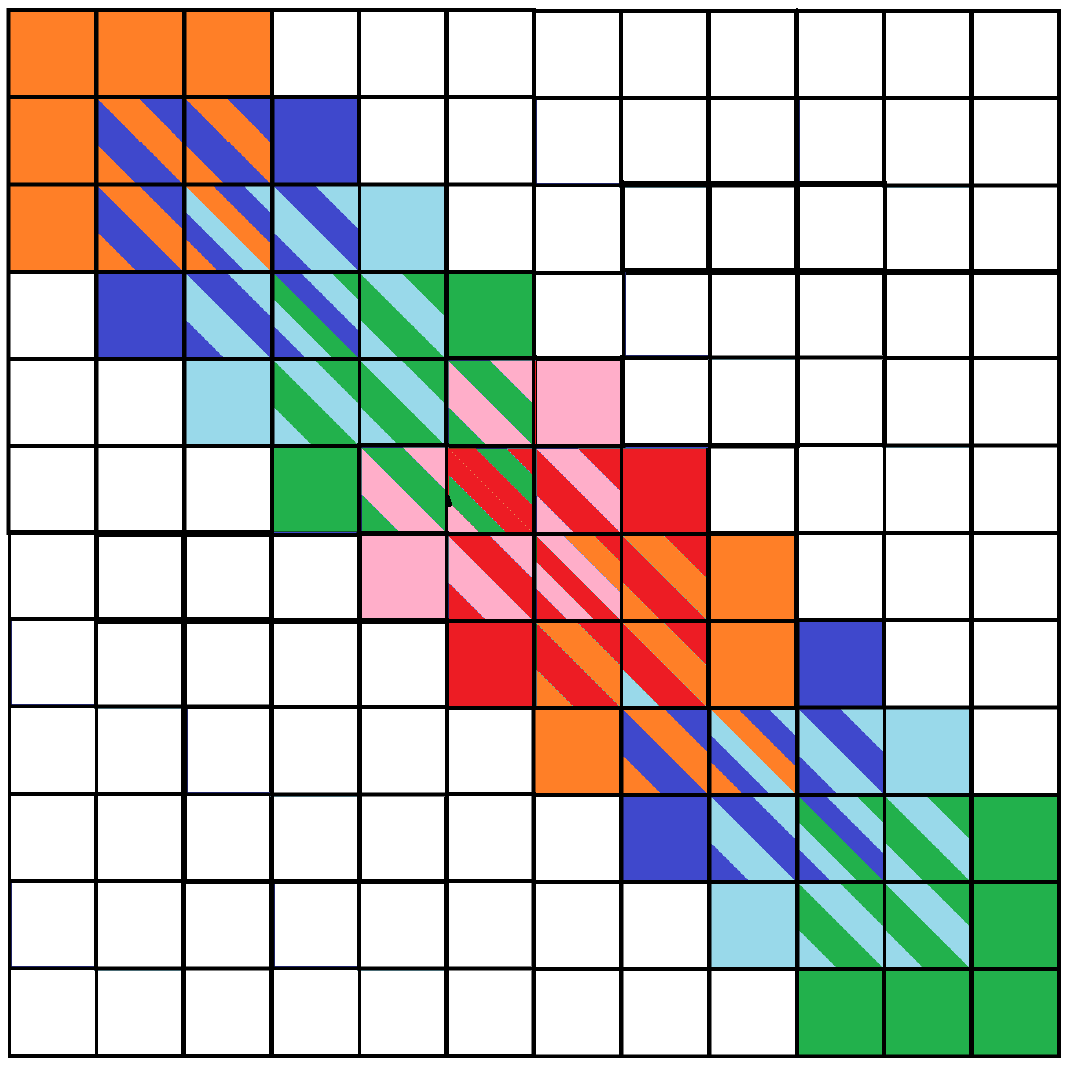
\includegraphics[width=1.1\textwidth]{img/partition}
      \caption{Partition of the problem matrix into sub-matrices}
    \end{figure}
  \end{column}

  \begin{column}{0.8\textwidth}
    \begin{figure}
      \centering
      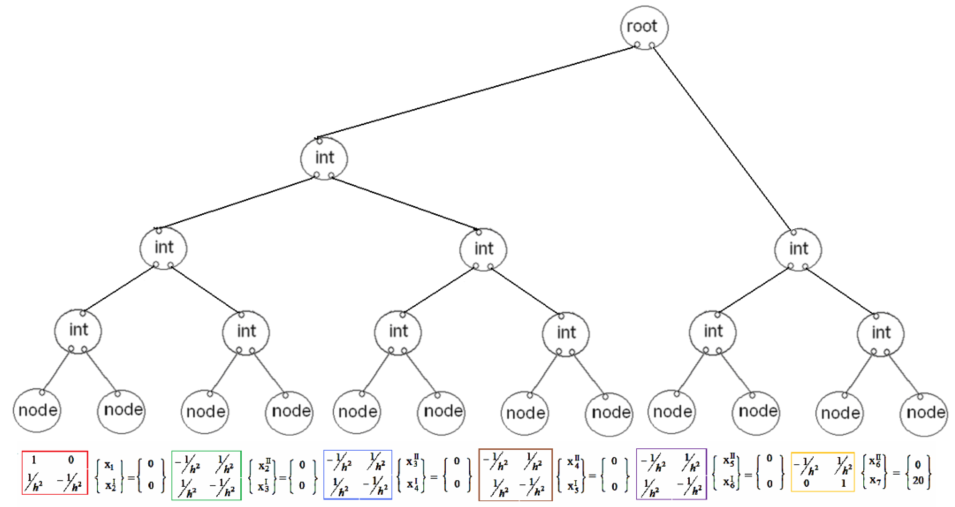
\includegraphics[width=0.95\textwidth]{img/tree_mat}
      \caption{Graph of matrices the solver will operate on}
    \end{figure}
  \end{column}
\end{columns}

\end{frame}
%%%%%%%%%%%%%%%%%%%%%%%%%%%

\begin{frame}{JAVA implementation (5/10) Productions}

We can identify a set of basic tasks applicable on any vertex. We call them \textbf{productions}. They can:
\begin{itemize}
  \item branch a vertex into two \{$P1$, $P2$\} or three \{$P3$\} child vertices
  \item initialize a vertex with particular coefficients \{$A1$, $A$, $AN$\}
  \item merge two vertices and eliminate unknowns -  \{$A2\_3$, $E1\_2\_5$, $A2\_2$, $E2\_2\_6$,$Aroot$, $Eroot$\} 
  \item backward substitute parts of solution - \{$BS\_2\_6$, $BS\_1\_5$\}
\end{itemize}

\end{frame}

%%%%%%%%%%%%%%%%%%%%%%%%%%%

\begin{frame}{JAVA implementation (6/10) Tree of tasks}

To obtain a solution for a 1-dimensional problem with 12 elements it is enough to execute the following productions, set by set, going from left to right, on respective vertices.

	\begin{figure}
      \centering
      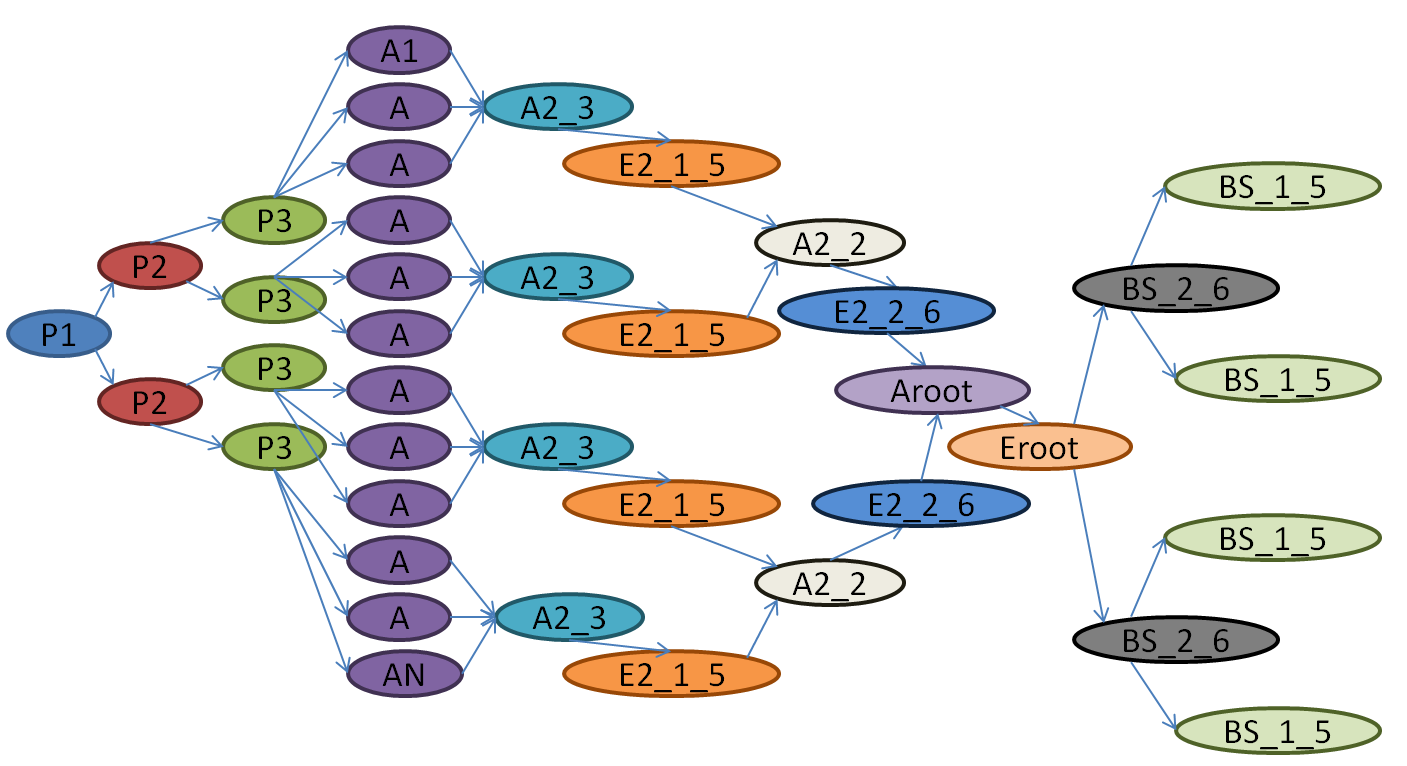
\includegraphics[width=1\textwidth]{img/task_tree}
    \end{figure}

\end{frame}
%%%%%%%%%%%%%%%%%%%%%%%%%%%

\begin{frame}{JAVA implementation (7/10) Flexibility}

We can solve any problem of size $3*2^{n-1}$ in one dimension. This is being done by repeating intermediate production sequence $n-2$ times.

\vskip 0.1in

For multidimensional problems we first solve in one direction and then use the results to construct the second tree. Its solution is solution to the master problem. We can do this for any dimension at a cost of having more right hand sides.

\vskip 0.1in

This \textbf{twofold scalability} greatly broadens the range of problems which can be solved using this technique. 

\end{frame}
%%%%%%%%%%%%%%%%%%%%%%%%%%%


\begin{frame}{JAVA implementation (8/10) Scalability}

Maximum of $6144x6144=37$ million elements in less than 3 minutes on 12-core machine with 12GB of RAM.

\vskip 0.1in

   \begin{figure}
      \centering
      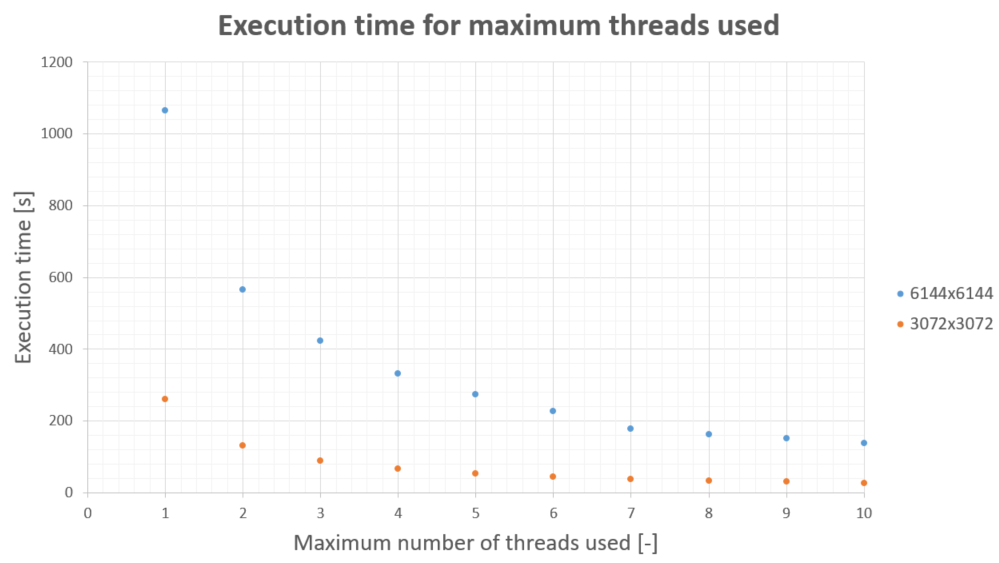
\includegraphics[width=1\textwidth]{img/perf}
    \end{figure}

\end{frame}
%%%%%%%%%%%%%%%%%%%%%%%%%%%


\begin{frame}{JAVA implementation (9/10) Testing}

The quality of software can be measured by how easy it is to test it.
\vskip 0.1in
In the implementation shown nearly everything can be tested in isolation - productions being the best example.
\vskip 0.1in
We can derive all levels of testing:
\begin{itemize}
  \item system - testing the algorithm against some well known problems
  \item integration - testing the algorithm against simple problems in single direction using a single thread
  \item unit - testing simplest tasks - mostly productions
\end{itemize}
\vskip 0.2in
This encourages to use well known and recognized techniques like Test Driven Development to create solutions to other problems.


\end{frame}
%%%%%%%%%%%%%%%%%%%%%%%%%%%


\begin{frame}{JAVA implementation (10/10) Conclusions}

What is a gain of using production based approach over classical procedural-style design?
\begin{itemize}
  \item \textbf{flexiblity} as we are able to solve any problem size in any dimensional space
  \item \textbf{performance} as productions are applied in parallel on every set of vertices
  \item \textbf{testability} as every production is an independent piece of code
  \item \textbf{readability} as production \textit{does one task and does it well}
\end{itemize}

\end{frame}
%%%%%%%%%%%%%%%%%%%%%%%%%%%

\begin{frame}{Thank you!}


Our research is funded by Polish National Science Centre \\ grant no. DEC-2015/19/B/ST8/01064

\end{frame}

%%%%%%%%%%%%%%%%%%%%%%%%%%%
%%%%%%%%%%%%%%%%%%%%%%%%%%%

\end{document}
